\chapter{\gls{coref_resolution_definition}}\label{ch:coreference-resolution}


\section{Background}\label{sec:background}
In linguistics, \gls{coref_definition} occurs when two or more expressions refer to the same person or thing \cite{Coreference}.
In the sample sentence of Fig.\ref{fig:coreferences}, the expression \emph{he} refers to a \gls{per} with the name \emph{Philip} and the word \emph{it} refers to the musical instrument \emph{bass}, a thing.

\begin{figure}[H]   %[h] puts picture right here. 't' stands for to, 'b' stands for bottom
    \centering
    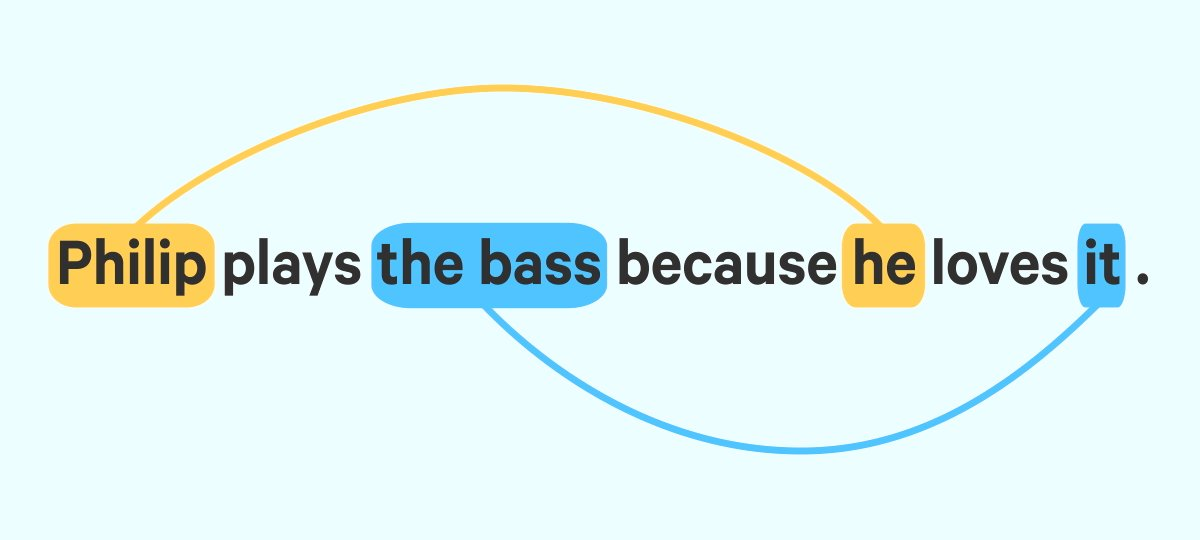
\includegraphics[width=0.7\textwidth]{Assets/spacycorefpic}
    \caption{Coreferences. Image from: \cite{spacy}}
    \label{fig:coreferences}
\end{figure}

\gls{coref_resolution_definition} is considered one of the most challenging tasks in \gls{nlp} and until recently was deemed an unsolved problem \cite{CorefResIsHard}.
The fundamental problem is the complex and ambiguous nature of natural language text, the requirement for a deep language understanding and the use of background knowledge in detecting \glspl{coref_definition} \cite{CorefResIsHard}.


\subsection{Definitions}\label{subsec:definitions}
In the sample sentence of Fig.\ref{fig:coreferences}, there are four \glspl{coref_mention} of which three are \glspl{token} [\emph{Philip, he, it}] and one is a \gls{span} [\emph{the bass}] consisting of more than one \gls{token}.
\glspl{coref_mention} often consist of long \glspl{span} such as \emph{The New York Times} or \emph{Bayerische Motoren Werke AG}.
Finding \glspl{coref_definition} in a text thus often is considered a \gls{span}-based task.
The \gls{coref_mention} \emph{Philip} is the \gls{coref_antecedent} for the \gls{coref_mention} \emph{it}.
As the name \emph{Philip} comes before \emph{it}, \emph{it} is the \gls{anaphora} for \emph{Philip}.
If \emph{Philip} came after \emph{it}, one would usually refer to \emph{it} as \gls{cataphora}.
The sample sentence has two \glspl{coref_cluster} or \gls{coref_definition} chains: [\emph{Philip, he}], [\emph{the bass, it}].

\subsection{Methods}\label{subsec:methods}
\subparagraph{Mention Detection}
The first step to detect \glspl{coref_definition} is \gls{coref_mention} detection \cite{StanfordNLPCoref}.
Earlier methods used grammatical parsers and named entity taggers on the text and, based on that, extracted
\glspl{span} that meet certain criteria as \gls{coref_mention}-candidates.
More recent \gls{coref_mention} detection systems go even further and extract literally all \gls{ngram} \glspl{span}
of \glspl{token} or words up to N=10, regardless of their grammatical attributes \cite{StanfordNLPCoref}.
Due to the computational complexity of this approach of
\begin{equation}
    O(number\_of\_tokens^4)
\end{equation}
for N=2 (Bi-Grams) \cite{CorefEndToEnd}, there is a need to filter out unlikely \glspl{span}.

\subparagraph{Rule Based Methods}
Earlier systems used rules to filter out non-coreferential pronouns like \emph{it} in sentences such as \emph{\underline{It} is likely that ...}.
These rule-based systems relied on regular expressions, dictionaries of key-verbs/-adjectives, \gls{pos} and \gls{ner} tags and other grammatical or syntactical rules.
Rule-based systems, however, generally underperform more modern systems that incorporate a learning process \cite{StanfordNLPCoref}.

\subparagraph{Feature Based Methods}
The next step thus were standard Machine Learning models that used decision trees, support vector machines and binary classifiers \cite{CorefSurvey}.
Theoretically, such models are capable to not only identify potential \glspl{coref_mention} but also whether such \glspl{coref_mention} are indeed \glspl{coref_definition}.
One common approach of such Classifiers is to implement a \emph{Mention-Pair-Architecture} that predicts if a given \gls{span} pair of an \gls{anaphora} and an \gls{coref_antecedent} are \glspl{coref_definition} or not \cite{StanfordNLPCoref}.
Another Classifier architecture type is the \emph{Mention-Rank-Architecture} that chooses the highest-scoring \gls{coref_antecedent} for each \gls{anaphora}.
\emph{Entity-based architectures} enhanced their feature set by adding \gls{coref_mention}-distances, syntactic, symantic, rule-based and lexical attributes to predict if a \gls{token} belongs to a certain \gls{coref_cluster} \cite{ClarkManning2015}.

Nevertheless, correctly detecting co-referential \glspl{coref_mention} remained difficult, mainly due to the model's lack for a deep language understanding \cite{StanfordNLPCoref}.

\subparagraph{Neural Network Based Methods}
A major breakthrough came with the advent of \glspl{llm} as contextual embeddings allowed to semantically compare \glspl{coref_mention}.
Consider the following phrases:

\begin{center}
    1: \textbf{Make a payment! You can make [it] in advance.} [anaphoric]
\end{center}
\begin{center}
    2: \textbf{Go west! You can make [it] in Hollywood.} [non-anaphoric]
\end{center}
\begin{center}
    Idea based on: \cite{StanfordNLPCoref}
\end{center}

Whereas the \emph{it} in the second phrase is non-anaphoric and part of the idiom \emph{make it}, the \emph{it} in the first phrase is anaphoric and refers to a \emph{payment}.
With contextual word-embeddings, the vectors for \emph{payment} and \emph{it} ideally should be similar in the first sentence whereas the vector for \emph{it} in the second sentence should significantly differ to any other word vector in that phrase.
The capability to detect the \glspl{coref_mention} \emph{payment} and \emph{it} as \glspl{coref_definition} should thus increase with contextual word embeddings.


\section{Models}\label{sec:models}
\gls{coref_definition} models can also be distinguished into three classes: Rule-Based, Pre-Trained and \gls{gen-llm} models.
As rule-based models factually are non-existent nowadays, the focus in the following chapter will be on Pre-Trained and \gls{gen-llm} models.

\subsection{Pre-Trained Models}\label{subsec:pre-trained-models}
\paragraph{Research}
All descriptions of the currently most performant pre-trained \gls{coref_definition} models are laid out in publicly available research papers.
Unfortunately, not all models are implemented in code and easily available as Python package.
This includes the two currently most performing \cite{CorefEvaluation} pre-trained \gls{coref_definition} models by Google Research \cite{CorefSeq2Seq} and Vladimir Dobrovolskii \cite{CorefDobrovolskii}.
As the model training of unimplemented \gls{coref_definition} research papers would go beyond the scope of this thesis,
I will shortly describe only those research papers for which a pre-trained Python package exists.

\subparagraph{e2e: End-to-end Neural \gls{coref_resolution_definition}}
In 2017, Lee et al.\cite{CorefEndToEnd} proposed an LSTM \cite{LSTM} model with a \emph{Mention-Rank-Architecture} where parsers and taggers are not required.
The model consists of two parts as shown in Fig.\ref{fig:e2e1} and \ref{fig:e2e2}:

\begin{figure}[H]   %[h] puts picture right here. 't' stands for to, 'b' stands for bottom
    \centering
    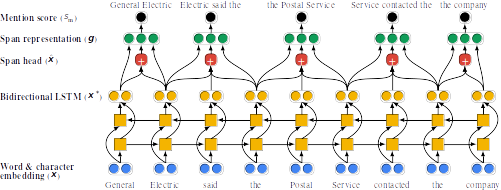
\includegraphics[width=1.0\textwidth]{Assets/e2e1}
    \caption{End-to-end Neural \gls{coref_resolution_definition}: Part 1}
    \label{fig:e2e1}
\end{figure}

In the first part (Fig.\ref{fig:e2e1}), the LSTM calculates \gls{span}-embeddings and assigns corresponding \gls{coref_mention} scores.
e2e is a supervised model trained with hand-labeled data.
Only the top M-ranked \glspl{span} with the highest \gls{coref_mention} scores are considered potential \glspl{coref_mention} and are further processed.
The concatenation of the \gls{token} embedding vectors creates the contextual \gls{span}-representation vectors.

\begin{figure}[H]   %[h] puts picture right here. 't' stands for to, 'b' stands for bottom
    \centering
    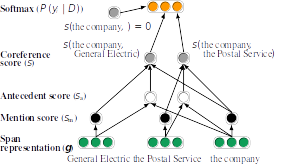
\includegraphics[width=0.7\textwidth]{Assets/e2e2}
    \caption{End-to-end Neural \gls{coref_resolution_definition}: Part 2}
    \label{fig:e2e2}
\end{figure}

In the second part of the model in Fig.\ref{fig:e2e2}, \emph{Antecedent scores} are computed from pairs of \gls{span}-representations.
The final \gls{coref_definition} \emph{score} is computed by summing the two \gls{coref_mention} \emph{scores} of the \glspl{span} and their pairwise \emph{Antecedent score}.
This calculation method avoids the computational inefficient evaluation of all (non-filtered-out) \gls{span} pairs and ensures, that the \gls{span}-pairs with the highest similarity yield the highest \gls{coref_definition} \emph{score}.

\subparagraph{c2f: Higher-order \gls{coref_resolution_definition} with Coarse-to-fine Inference}
In 2018, Lee et al. further improved their own model by changing the inference procedure of the \emph{Mention-Rank-Architecture}\cite{CorefCoarseFine} to refine \gls{span} representations.
This improved both, the computational complexity and the performance of the model.

\subparagraph{BERT for \gls{coref_resolution_definition}}
In 2019, Joshi et al. \cite{CorefWithBert} reused the \emph{Mention-Rank-Architecture} of Lee et al.\cite{CorefEndToEnd} but substituted the LSTM-embeddings with \gls{BERT}-embeddings \cite{BERT} and later with \gls{SpanBERT}-embeddings \cite{SpanBERT}.
\gls{SpanBERT} was designed to better represent \glspl{span} of text and is a pre-training method that extends the \gls{BERT}-model by masking contiguous random \glspl{span}, rather than random \glspl{token} \cite{SpanBERT}.
\gls{SpanBERT} is applicable to a wide range of tasks such as question answering, relation extraction and \gls{coref_resolution_definition}.
For their Coreference-model, they applied the \gls{SpanBERT}-method on a \gls{coref_definition} task and a \gls{coref_definition} training set \cite{SpanBERT}.
The model achieves an F1-score of 77.7 for the \gls{SpanBERT}-base and 79.6 for the \gls{SpanBERT}-large \cite{CorefWithBert}, currently ranking among the five best \gls{coref_resolution_definition} models \cite{CorefEvaluation}.

\subparagraph{s2e: \gls{coref_resolution_definition} without \gls{span} Representations}
In 2021, Kirstain et al.\cite{KirstainCoref} came up with a different architecture that focused on \glspl{token} instead of \glspl{span}.

\begin{figure}[H]   %[h] puts picture right here. 't' stands for to, 'b' stands for bottom
    \centering
    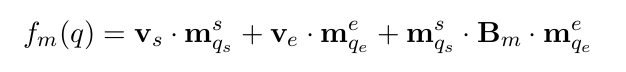
\includegraphics[width=0.7\textwidth]{Assets/Kirstain1}
    \caption{Bilinear function: start/end Mention embeddings: \textbf{m}\textsuperscript{s}, \textbf{m}\textsuperscript{e}}
    \label{fig:s2e1}
\end{figure}
The model computes \gls{coref_mention} scores as bi-affine products over the start and end \gls{token} representations (\textbf{m}\textsuperscript{s}, \textbf{m}\textsuperscript{e}) with
\textbf{v}\textsubscript{s}, \textbf{v}\textsubscript{e} and \textbf{B}\textsubscript{m} as trainable matrices (Fig.\ref{fig:s2e1}).
\begin{figure}[H]   %[h] puts picture right here. 't' stands for to, 'b' stands for bottom
    \centering
    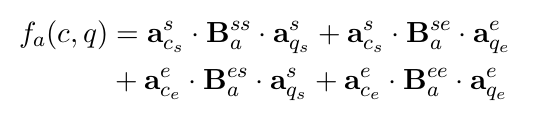
\includegraphics[width=0.6\textwidth]{Assets/Kirstain2}
    \caption{Bilinear function: start/end Antecedent embeddings:  \textbf{a}\textsuperscript{s}, \textbf{a}\textsuperscript{e}}
    \label{fig:s2e2}
\end{figure}
Similarly, it also extracts start and end \gls{token} representations (\textbf{a}\textsuperscript{s}, \textbf{a}\textsuperscript{e}) for
the antecedent scoring function with \textbf{B}\textsubscript{m} as another trainable matrix (Fig.\ref{fig:s2e2}).
This calculation is equivalent to computing a bilinear transformation between the concatenation of each \gls{span}’s boundary \glspl{token}’ representations,
but bypasses the need to create n\textsuperscript{2} explicit \gls{span} representations (for Bi-Gram \gls{span}) und thus reduces complexity \cite{KirstainCoref}.
The model is the fastest of all known \gls{coref_definition} models and, with an F1-score of 80.4, currently ranks fourth \cite{CorefEvaluation} in regard to prediction performance.

\paragraph{Available Models}
Based on these research papers, the following Python modules are available:

\subparagraph{AllenNLP}
AllenNLP \cite{AllenNLP} is an AI platform supported by the Allen Institute for Artificial Intelligence \cite{AllenAI}.
AllenNLP offers multiple pre-trained models and a pip-installable Python module \cite{AllenNLP}.
Among the models offered is a pre-trained \gls{coref_resolution_definition} model that is based on the c2f-model by Lee et al.\cite{CorefCoarseFine}.
The GloVe embeddings in the original paper \cite{CorefCoarseFine} have been substituted with \gls{SpanBERT} embeddings \cite{AllenNLPCorefModel}.
Unfortunately, since 2022 the AllenNLP ecosystem is in maintenance mode.
Dependencies to more recent Python versions are not upgraded and the most recent training for the \emph{coref-spanbert-large}-model goes back to March 2021.
Additionally, AllenNLP only offers pre-trained models for English but not for German.

\subparagraph{F-COREF}
F-COREF is a Python implementation and an adopted version of the s2e-model by Kirstain et al. \cite{KirstainCoref}.
F-COREF predicts \glspl{coref_cluster} 29 times faster than the AllenNLP model and requires only 15\% of its GPU memory use, with only a small
drop in performance (78.5 vs 79.6 average F1) \cite{FastCoref}.
Unfortunately, F-COREF currently only has a pre-trained model for English but not for German.

\subparagraph{Coreferee}
Coreferee \cite{Coreferee} is a pip-installable Python package that uses a mixture of \glspl{ann} and programmed language-specific rules.
It focuses heavily on detecting \glspl{anaphora} and noun phrases and thus depends on the grammatical and syntactical capabilities of spacy \cite{spacy}.
The likelihood scores for anaphoric pairs are calculated by utilizing the contextualized vectors of the underlying and pre-trained spacy models.
Specific language packages other than English exist for German, Polish and French and must be downloaded individually.

\subparagraph{Crosslingual-Coreference}\label{subpar:crosslingual-coreference}
The Crosslingual-Coreference model \cite{xxCoref} builds on the AllenNLP-Coreference model \cite{AllenNLPCorefModel} but modifies its \emph{coref\_resolved}-method.
It investigates all the \glspl{coref_cluster} found by the AllenNLP-Coreference model, but only considers \glspl{coref_cluster} that contain a noun phrase \cite{AllenCorefModelModification}.
To determine if a \gls{coref_cluster} contains a noun phrase, it uses the \gls{pos}-tagger of pre-trained models from spacy \cite{spacy} that are also available in languages other than English.
If the model parameter is set to \emph{minilm}, the \gls{llm} used in resolving \glspl{coref_cluster} is multilingual and pre-trained by Microsoft \cite{xxCorefMinilmModel}.
As such, this model can be applied multilingual, i.e. to English and German.

\paragraph{Evaluated Pre-Trained Models}
As only the Coreferee \cite{Coreferee} and Crosslingual-Coreference model \cite{xxCoref} are available for the German language, in the project only those two pre-trained models were evaluated against each other.
I tried both extensively with multiple texts, and the Crosslingual-Coreference model \cite{xxCoref} clearly outperformed the Coreferee \cite{Coreferee} model.
It found more \gls{coref_definition} mentions and had a lower entity confusion rate in texts that contained multiple entities.
The Crosslingual-Coreference model \cite{xxCoref} was later compared against a \gls{gen-llm} approach.

\subsection{\gls{gen-llm} Models}\label{subsec:generative-llm-models}
\paragraph{Pre-Trained AND Generative}\label{par:pretrained-and-gen-llm}
Besides using \glspl{gen-llm} and \gls{prompt} requests directly, there are also dedicated architectures and indirect ways to extract \glspl{coref_definition} from text.
In the previous section, the \gls{coref_definition} model by Google Research \cite{CorefSeq2Seq} was classified as a pre-trained model, but it could also be classified as a \gls{gen-llm} model as the boundaries between these two types are increasingly blurry.

The pre-trained Google model \cite{CorefSeq2Seq} is a sequence-to-sequence model that uses both stacks of the \gls{Transformer} architecture, i.e. the encoder \emph{and} the decoder.
It so generates new text based on an input sequence where the input sequence is an untagged string and the output sequence the input string plus tags attached to it.
The tags contain the desired \gls{coref_definition} annotations.
The model is trained with the aim to annotate the input string with the respective \gls{coref_definition} tags.

This approach is very similar to the one Wang et al \cite{gptner} use in their model for the \gls{ner} task (see \ref{subsec:deep-learning-models}).

Whereas the Google \cite{CorefSeq2Seq} model introduces some extra layers to an encoder-decoder stack, Zhang et al \cite{zhangcorefseq2seq} use a plain pre-trained encoder-decoder (text-to-text) T5 model \cite{googlet5} and finetune it in a supervised way with annotated examples.
The source sequence contains the input string and the target sequence the \emph{\gls{coref_definition}-annotated} input string.
During finetuning, the classification task uses the usual source-target sequence pair and tries to minimize the cross-entropy loss given the per-\gls{token} labels \cite{zhangcorefseq2seq}.
\paragraph{Models used}
As stated previously, neither the Google \cite{CorefSeq2Seq} model nor the Zhang et al \cite{zhangcorefseq2seq} model are (easily) available as a Python module.
I therefore tested the \gls{gen-llm} approach directly as described in the next section.

\section{Code Implementation}
\subsection{Implementation of Pre-Trained Model}
As stated previously (see Section \ref{subpar:crosslingual-coreference}), the Crosslingual-Coreference model \cite{xxCoref} is based on the deprecated AllenNLP-Coreference model \cite{AllenNLPCorefModel}, depends on the \gls{pos}-tagger from a certain spacy version and uses a fine-tuned and pre-trained Microsoft \gls{llm} that was last updated in 2021.
It has some issues for Python versions greater than 3.10 and dependency conflicts to other Python libraries in the project that could not be resolved.


I thus decided to run the Crosslingual-Coreference model \cite{xxCoref} in an isolated environment using Docker.
The files for building the Docker container can be found in the \emph{/src/D\_coref/img\_xx\_coref\_files} directory that also contains a Dockerfile and a requirements.txt file.
The Docker container is accessible by using http requests.

The Crosslingual-Coreference model \cite{xxCoref} in the Docker container is run as a spacy pipeline-component that attaches found \glspl{coref_cluster} to spacy's Doc-object custom extensions.
The \glspl{coref_cluster} are nested Python lists in the format
\begin{center}
\scriptsize\textbf{{[[[cl1\_start1, cl1\_end1], [cl1\_start2, cl1\_end2]], [[cl2\_start1, cl2\_end1], [cl2\_start2, cl2\_end2]]]}}
\end{center}
where character start and end index positions for each word in a \gls{coref_cluster} are shown.

The function \emph{spread\_comp\_ext\_to\_coref\_cluster\_spans()} in Python-Code \ref{code:spread-comp-ext-to-coref-cluster-spans}

\begin{listing}[H]
    \captionof{listing}{spread\_comp\_ext\_to\_coref\_cluster\_spans()}
    \inputminted[
    firstline=348,
    lastline=369,
    firstnumber=348,
    ]{python}{/media/rainergo/PROJECTS/UASFRA-MS-Thesis/src/B_spacy_pipeline/spacy_pipe_funcs.py}
    \label{code:spread-comp-ext-to-coref-cluster-spans}
\end{listing}
first checks if any \gls{coref_cluster} word overlaps with a spacy custom extension \gls{span} that has a company name and company symbol attached to it.
If this is the case, it creates a new instance of the SearchMatch class with the same company name and company symbol for every other member of the \gls{coref_cluster}.

Before setting the found \glspl{coref_definition} to the spacy custom extensions, the function \emph{resolve\_span\_conflicts\_and\_set\_new\_ents()} in Python-Code \ref{code:resolve-span-conflicts-and-set-new-ents}
\begin{listing}[H]
    \captionof{listing}{resolve\_span\_conflicts\_and\_set\_new\_ents()}
    \inputminted[
    firstline=92,
    lastline=127,
    firstnumber=92,
    ]{python}{/media/rainergo/PROJECTS/UASFRA-MS-Thesis/src/B_spacy_pipeline/spacy_pipe_funcs.py}
    \label{code:resolve-span-conflicts-and-set-new-ents}
\end{listing}

checks if the respective spacy \gls{token} or \gls{span} already has these extensions set by the previous \gls{ner} component of the pipeline.
Only if this is not the case, the custom extension is set with the information from the SearchMatch instances.

\subsection{Implementation of \gls{gen-llm} Model}\label{subsec:langchain-explain}
To implement the \gls{gen-llm} model directly as reasoned in Section \ref{par:pretrained-and-gen-llm}, the Python LangChain \cite{LangChain} library was used.
LangChain is a modular LLM framework where components such as \glspl{prompt}, \glspl{llm}, Agents and Tools can be chained together to build an \gls{llm} pipeline.

The latest LangChain version 0.3 uses Pydantic version 2 \cite{Pydantic}, a mandatory type checking library, that had unresolvable dependency conflicts with existing libraries in the project.
For this reason, I also isolated the \gls{gen-llm} approach by using Docker.
The files for building the Docker container can be found in the \emph{/src/D\_coref/img\_llm\_extract\_coref\_files} directory that, among other files, contains a Dockerfile and a requirements.txt file.

\paragraph{Data Model}\label{par:coref-data-model}
In the mentioned directory, there is also a Python file named \emph{data\_models.py} (see Python-Code \ref{code:data-model-coref-llm-extract}) that lays out the desired format of the \gls{llm} response and the format of messages in the \gls{prompt}.
This is important because \gls{gen-llm}s usually suffer to deliver the generated text response in an appropriate format such as JSON so that it can be further processed by an algorithm.

\begin{listing}[H]
    \captionof{listing}{Data Model Coref LLM Extract}
    \inputminted[
    firstline=4,
    lastline=36,
    firstnumber=4,
    ]{python}{/media/rainergo/PROJECTS/UASFRA-MS-Thesis/src/D_coref/img_llm_extract_coref_files/data_models.py}
    \label{code:data-model-coref-llm-extract}
\end{listing}

Python-Code \ref{code:data-model-coref-llm-extract} shows the data model which consists of four Python classes that all inherit from Pydantic's \emph{BaseModel}.
This way, Pydantic in the background checks instances of these classes for their type (such as Integer, Float, String, etc.) and raises an error if the value of the respective instance variable does not comply with it.

\subparagraph{\gls{prompt}}
The \gls{prompt} for the \gls{gen-llm} model contains examples (few-shots) in the form of instances of these Pydantic classes.
Instances of the class Cluster contain the article text, an instance of the class ClusterHead and potentially multiple instances of the class Coreference.

Instances of the ClusterHead class are created with the information that was previously extracted by the pipeline's \gls{ner} component: the company name (\emph{head\_text}) and the start (\emph{head\_index\_start}) and end (\emph{head\_index\_end}) position of this company name within the article text.

Instances of the class \gls{coref_definition} contain the \gls{coref_definition} string (\emph{coref\_text}) and the \gls{coref_definition} string with two words on the right and left (\emph{coref\_with\_surroundings}).


As an example, let's say that the article text is

\begin{center}
    \textbf{Siemens manufactures trains. It is located in Munich.}
\end{center}
then the according few-shot example in the \gls{prompt} would be

\begin{center}
\scriptsize\textbf{{
Cluster(cluster\_id=1, text="Siemens manufactures trains. It is located in Munich.",\newline
        cluster\_head=ClusterHead(head\_text="Siemens", head\_index\_start=0, head\_index\_end=7),\newline
        coreferences=[Coreference(coref\_text="It", coref\_with\_surroundings="manufactures trains. It is located")])}}
\end{center}

The question is why the \gls{coref_definition} class does not include position indexes of the found \gls{coref_definition} word within the text similar to the \emph{head\_index\_start} and \emph{head\_index\_end} variables for the company name.
Then the subsequent algorithm could easily locate the \gls{coref_definition} words in the text and attach them to the respective custom extensions of the Doc-object in the spacy pipeline.

I tried to force the \gls{gen-llm} to return those position integer values for \glspl{coref_definition} it found but the model, even equipped with the respective tools in the LangChain pipeline, did not succeed.
I assume that this could also be the reason why Wang et al \cite{gptner} had their \gls{ner} model generate string annotations instead of returning text position indexes such as

\begin{center}
    \emph{@@Columbus\#\# is a city}
\end{center}
for the input sequence \emph{Columbus is a city} (see Section \ref{par:gpt-ner}).

I also could have asked the \gls{gen-llm} to annotate the \gls{coref_definition} it found with the same symbols such as:
\begin{center}
    \textbf{Siemens manufactures trains. @@It\#\# is located in Munich.}
\end{center}

But the problem was that the article text, even after cleaning, already contained such symbols (i.e.\emph{@} and\emph{\#}) so that a subsequent algorithm could potentially have confused them.

The few-shot examples provided to the \gls{gen-llm} can be found in: \newline
\emph{src/D\_coref/img\_llm\_extract\_coref\_files/examples.py}

\subparagraph{Response Format}
The Pydantic classes are not only used for few-shot examples in the \gls{prompt}, but also for defining the response format.
The LangChain pipeline or chain is defined in \newline
\emph{src/D\_coref/img\_llm\_extract\_coref\_files/coref\_langchain.py}:

\begin{listing}[H]
    \captionof{listing}{LangChain pipeline for COREF}
    \inputminted[
    firstline=19,
    lastline=40,
    firstnumber=19,
    ]{python}{/media/rainergo/PROJECTS/UASFRA-MS-Thesis/src/D_coref/img_llm_extract_coref_files/coref_langchain.py}
    \label{code:langchain-coref}
\end{listing}

The LangChain chain is built in line 26 of the above code and connects a filled PromptTemplate with an \gls{llm} module, in this case OpenAI's ChatOpenAI module running their \textbf{gpt-4o} model.

In line 25, the ChatOpenAI module via the function
\begin{center}
\emph{with\_structured\_output(schema=Cluster)}
\end{center}
is bound to Pydantic's Cluster class, as discussed previously.
This forces the \gls{llm} to return its response in a format that is compliant with that class.
As the \gls{gen-llm} approach is run via a Docker container and http requests, the Pydantic class instances are converted to serializable Python dictionaries and \gls{json} and back to Pydantic class instances in the process.

\subparagraph{Processing the LLM Response}
Ideally, the response from the \gls{llm} is in the desired format and, among other information, contains the values for the variables \emph{coref\_text} and \emph{coref\_with\_surroundings}.
They will now be converted to values that can be attached as custom extensions in the Doc-object of the spacy pipeline by the following function:

\begin{listing}[H]
    \captionof{listing}{Convert LLM response to Matches}
    \inputminted[
    firstline=418,
    lastline=445,
    firstnumber=418,
    fontsize=\tiny,
    ]{python}{/media/rainergo/PROJECTS/UASFRA-MS-Thesis/src/B_spacy_pipeline/spacy_pipe_funcs.py}
    \label{code:llm-to-match}
\end{listing}

The \gls{coref_definition} position index within the text are determined by using \gls{Regex} functions and patterns.

First, the position indexes of the \emph{coref\_with\_surroundings} text within the article text, and afterward the \emph{coref\_text} within the \emph{coref\_with\_surroundings} text are determined.
A \gls{Regex} search for the \emph{coref\_text} in the article text \underline{alone} would not be sufficient,
because the \emph{coref\_text} could be a common word such as \emph{it}, which might occur multiple times in the text without being a \gls{coref_definition}.
The two required words to the left and right of the actual \gls{coref_definition} word ensure a text sequence of at least five \glspl{token} which is unlikely to occur twice in the given article text.

The process for each \gls{coref_definition} yields a Python \emph{re Match object} that contains the start and end index of the \emph{coref\_text} within the article text.

Before the information is attached to the \gls{token} or \gls{span} custom extensions of the Doc-object, the function \emph{resolve\_span\_conflicts\_and\_set\_new\_ents()} again checks if there is an overlap with custom extension values that were already set by the previous \gls{ner} pipeline component (see: Python-Code \ref{code:resolve-span-conflicts-and-set-new-ents}).

\subparagraph{Collecting Entities}
Once the spacy pipeline has run, the company information stored in the custom extensions, is collected.


It could be that a news article contains multiple sentences each mentioning multiple companies.
The functions
\begin{center}
    \emph{get\_ents\_with\_custom\_extension()} and \emph{get\_sentences\_with\_custom\_extensions()}
\end{center}
collect the company information fom the custom extensions in the spacy Doc-object and store them in a Python dictionary:

\begin{listing}[H]
    \captionof{listing}{Collection of custom extension information}
    \inputminted[
    firstline=49,
    lastline=63,
    firstnumber=49,
    fontsize=\tiny,
    ]{python}{/media/rainergo/PROJECTS/UASFRA-MS-Thesis/src/B_spacy_pipeline/spacy_pipe_funcs.py}
    \label{code:collect-entities}
\end{listing}

They make sure that multiple company mentions in a sentence are accounted for.
The resulting nested Python list of dictionaries is compiled for every article containing company information and structurally looks like this sample:

\begin{listing}[H]
    \captionof{listing}{Company information for article text}
    \inputminted[
    firstline=1,
    lastline=39,
    firstnumber=1,
    ]{python}{/media/rainergo/PROJECTS/UASFRA-MS-Thesis/doc/Assets/after_ner_coref.json}
    \label{code:dict-after-coref-and-ner}
\end{listing}

Sentences that contain more than one company mention within each dictionary store the information in another list of Python dictionaries.
For sentences that contain only one company mention, this list only contains one item.

\paragraph{Topic Sentences}\label{par:topic-sents}
The news articles are stored in a parquet file to be converted to a pandas DataFrame as described in Section \ref{ch:project_setup}.
Each row in the DataFrame contains one article and each list of Python dictionaries, as shown in the Python-Code \ref{code:dict-after-coref-and-ner}, is stored in one cell of the \emph{ner\_coref} column as object.\\

To do Topic Modelling on sentences as described in the next chapter, the nested list of Python dictionaries (Python-Code \ref{code:dict-after-coref-and-ner}) must be flattened first to have one sentence in each row of the DataFrame.
This is what the
\begin{center}
\emph{convert\_nested\_ner\_coref\_dict()}
\end{center}
function in the Python file \emph{main\_process.py} does:

\begin{listing}[H]
    \captionof{listing}{Un-Nesting \gls{ner} and COREF Information}
    \inputminted[
    firstline=78,
    lastline=84,
    firstnumber=78,
    ]{python}{/media/rainergo/PROJECTS/UASFRA-MS-Thesis/main_process.py}
    \label{code:unnest-dict-after-coref-and-ner}
\end{listing}

Before inserting new rows into the DataFrame, the function in line 80 inserts a new \emph{art\_id} column that is just the row index of the DataFrame.
As each row contains just one article, the new column preserves the article identification of the soon-to-be expanded DataFrame.
The pandas DataFrame function \emph{explode} in line 51 then creates new rows for each dictionary (shown in Python-Code \ref{code:dict-after-coref-and-ner})
and pandas \emph{string accessor} method in line 52 finally inserts the sentences into the new column \emph{top\_sent}.

\subsection{Comparing Pre-Trained vs. \gls{gen-llm} approach}
The \gls{gen-llm} approach outperforms the pre-trained Crosslingual-Coreference model \cite{xxCoref} on the sample text I tested them with.
The latter model performs well if the article text mentions only one company, but links \glspl{coref_definition} to the wrong company if multiple companies are mentioned.
Here, the pre-trained Crosslingual-Coreference model \cite{xxCoref} might show its lack for contextual understanding as the underlying \gls{llm} is only used for finding and resolving \glspl{coref_cluster} (see: Section \ref{subpar:crosslingual-coreference}).
The \gls{gen-llm} is not perfect either as it does not find all \glspl{coref_definition}, but those that are found are mostly correct.
In addition, the \gls{gen-llm} was only provided with four few-shot examples in the \gls{prompt} and adding more examples would probably improve the model further.
I thus have decided to use the \gls{gen-llm} approach for the task of \gls{coref_definition} resolution.

\subsection{Information Extraction Pipeline}
After the \gls{coref_resolution_definition} component has run, the spacy pipeline has attached the found company information to the respective custom extensions
that in a subsequent step will be stored as a list of dictionaries as shown in Python-Code \ref{code:dict-after-coref-and-ner}:
\begin{figure}[H]   %[h] puts picture right here. 't' stands for to, 'b' stands for bottom
    \centering
    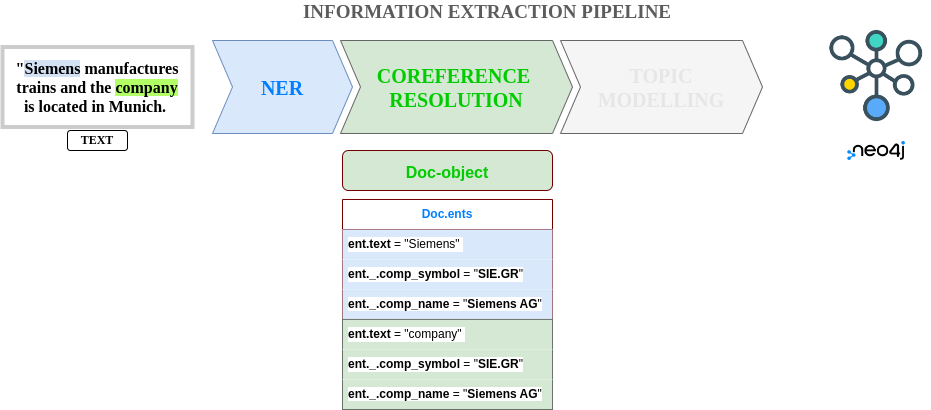
\includegraphics[width=0.85\textwidth]{Assets/pipelineCoref}
    \caption{spacy pipeline after COREF component}
    \label{fig:pipeCoref}
\end{figure}
In the example, it contains the company name \emph{Siemens} coming from the \gls{ner} component and the \gls{coref_definition} \emph{company} coming from the Coreference Resolution component.
















